
In his novel paper \cite{Purcell1977}, Purcell treats for the first time the issue of swimming on a microscopic level and the principal problems linked to it. He especially illustrates, why any micro-organism trying to swim using a reciprocal movement like the one of a scallop, i.e. swimming by opening and closing a valve, cannot move. This observation, also known as the \emph{scallop theorem}\footnote{For a proof as well as an elementary introduction to the topic we refer to the encyclopedia article \cite{DeSimone2011}.} entails the problem of finding the simplest swimming mechanism at microscopic scales; that is, the capacity to advance using a periodic change of  shape - a swimming \emph{stroke} - in  the absence of external forces. A variety of such mechanisms has already been proposed and analyzed, see e.g. \cite{Alouges2013, Najafi2004, Purcell1977}.


The principal mathematical challenge of this problem stems from the low value of the Reynolds number $\re = \rho u L/\mu$ which gives an estimate of the relative importance of inertial to viscous forces for an object of characteristic length scale $L$ moving at speed $u$ through a Newtonian fluid of density $\rho$ and dynamic viscosity $\mu$. In the low Reynolds number regime, i.e. $\re \ll 1$, the inertial forces become irrelevant and consequently, micro-swimmers can only utilize the viscous resistance of the surrounding fluid to move. In mathematical terms, the micro-swimmers are governed by the steady Stokes equations, which are linear and symmetric under time reversal. In the case of the scallop, this means that whatever forward motion is caused by closing its valves, it will exactly be compensated by the movement produced by reopening them, regardless of the speed of these two processes.

Let us formulate the basic problem of swimming: given a periodic record of shape changes of a swimmer, predict the corresponding history of positions and orientations in space. A closely related question is the one of \emph{controllability}; that is, whether it is possible to achieve any prescribed position and orientation in space starting from an arbitrary initial position and orientation using an appropriate sequence of shape deformations. In fact, the peculiarity of swimming at low values of $\re$ stems from the fact that reciprocal shape changes cannot contribute to the net displacement as inertial forces are negligible. This especially becomes an issue when we only have few control variables at our disposal. Indeed, the scallop theorem actually shows that swimmers with only one control variable are not controllable.

Once the controllability of a swimmer is assured, the natural follow-up question is to ask which swimming strokes achieve a prescribed net displacement with the lowest energy consumption. In other words, mathematically speaking, we face an \emph{optimal control problem}. From the point of view of biology, this is relevant in the light of \emph{natural selection} among micro-organisms, whereas from the engineering standpoint, this is crucial since, as it is pointed out in \cite{Avron2004}, if a micro-swimmer should have an effect on macroscopic scales, it has to swim faster than bacteria and therefore consumes $10^4$ more energy than a bacterium. Hence, it is desirable to know the most effective swimming strokes for a micro-swimmer.

\begin{figure}[h]
\centering
	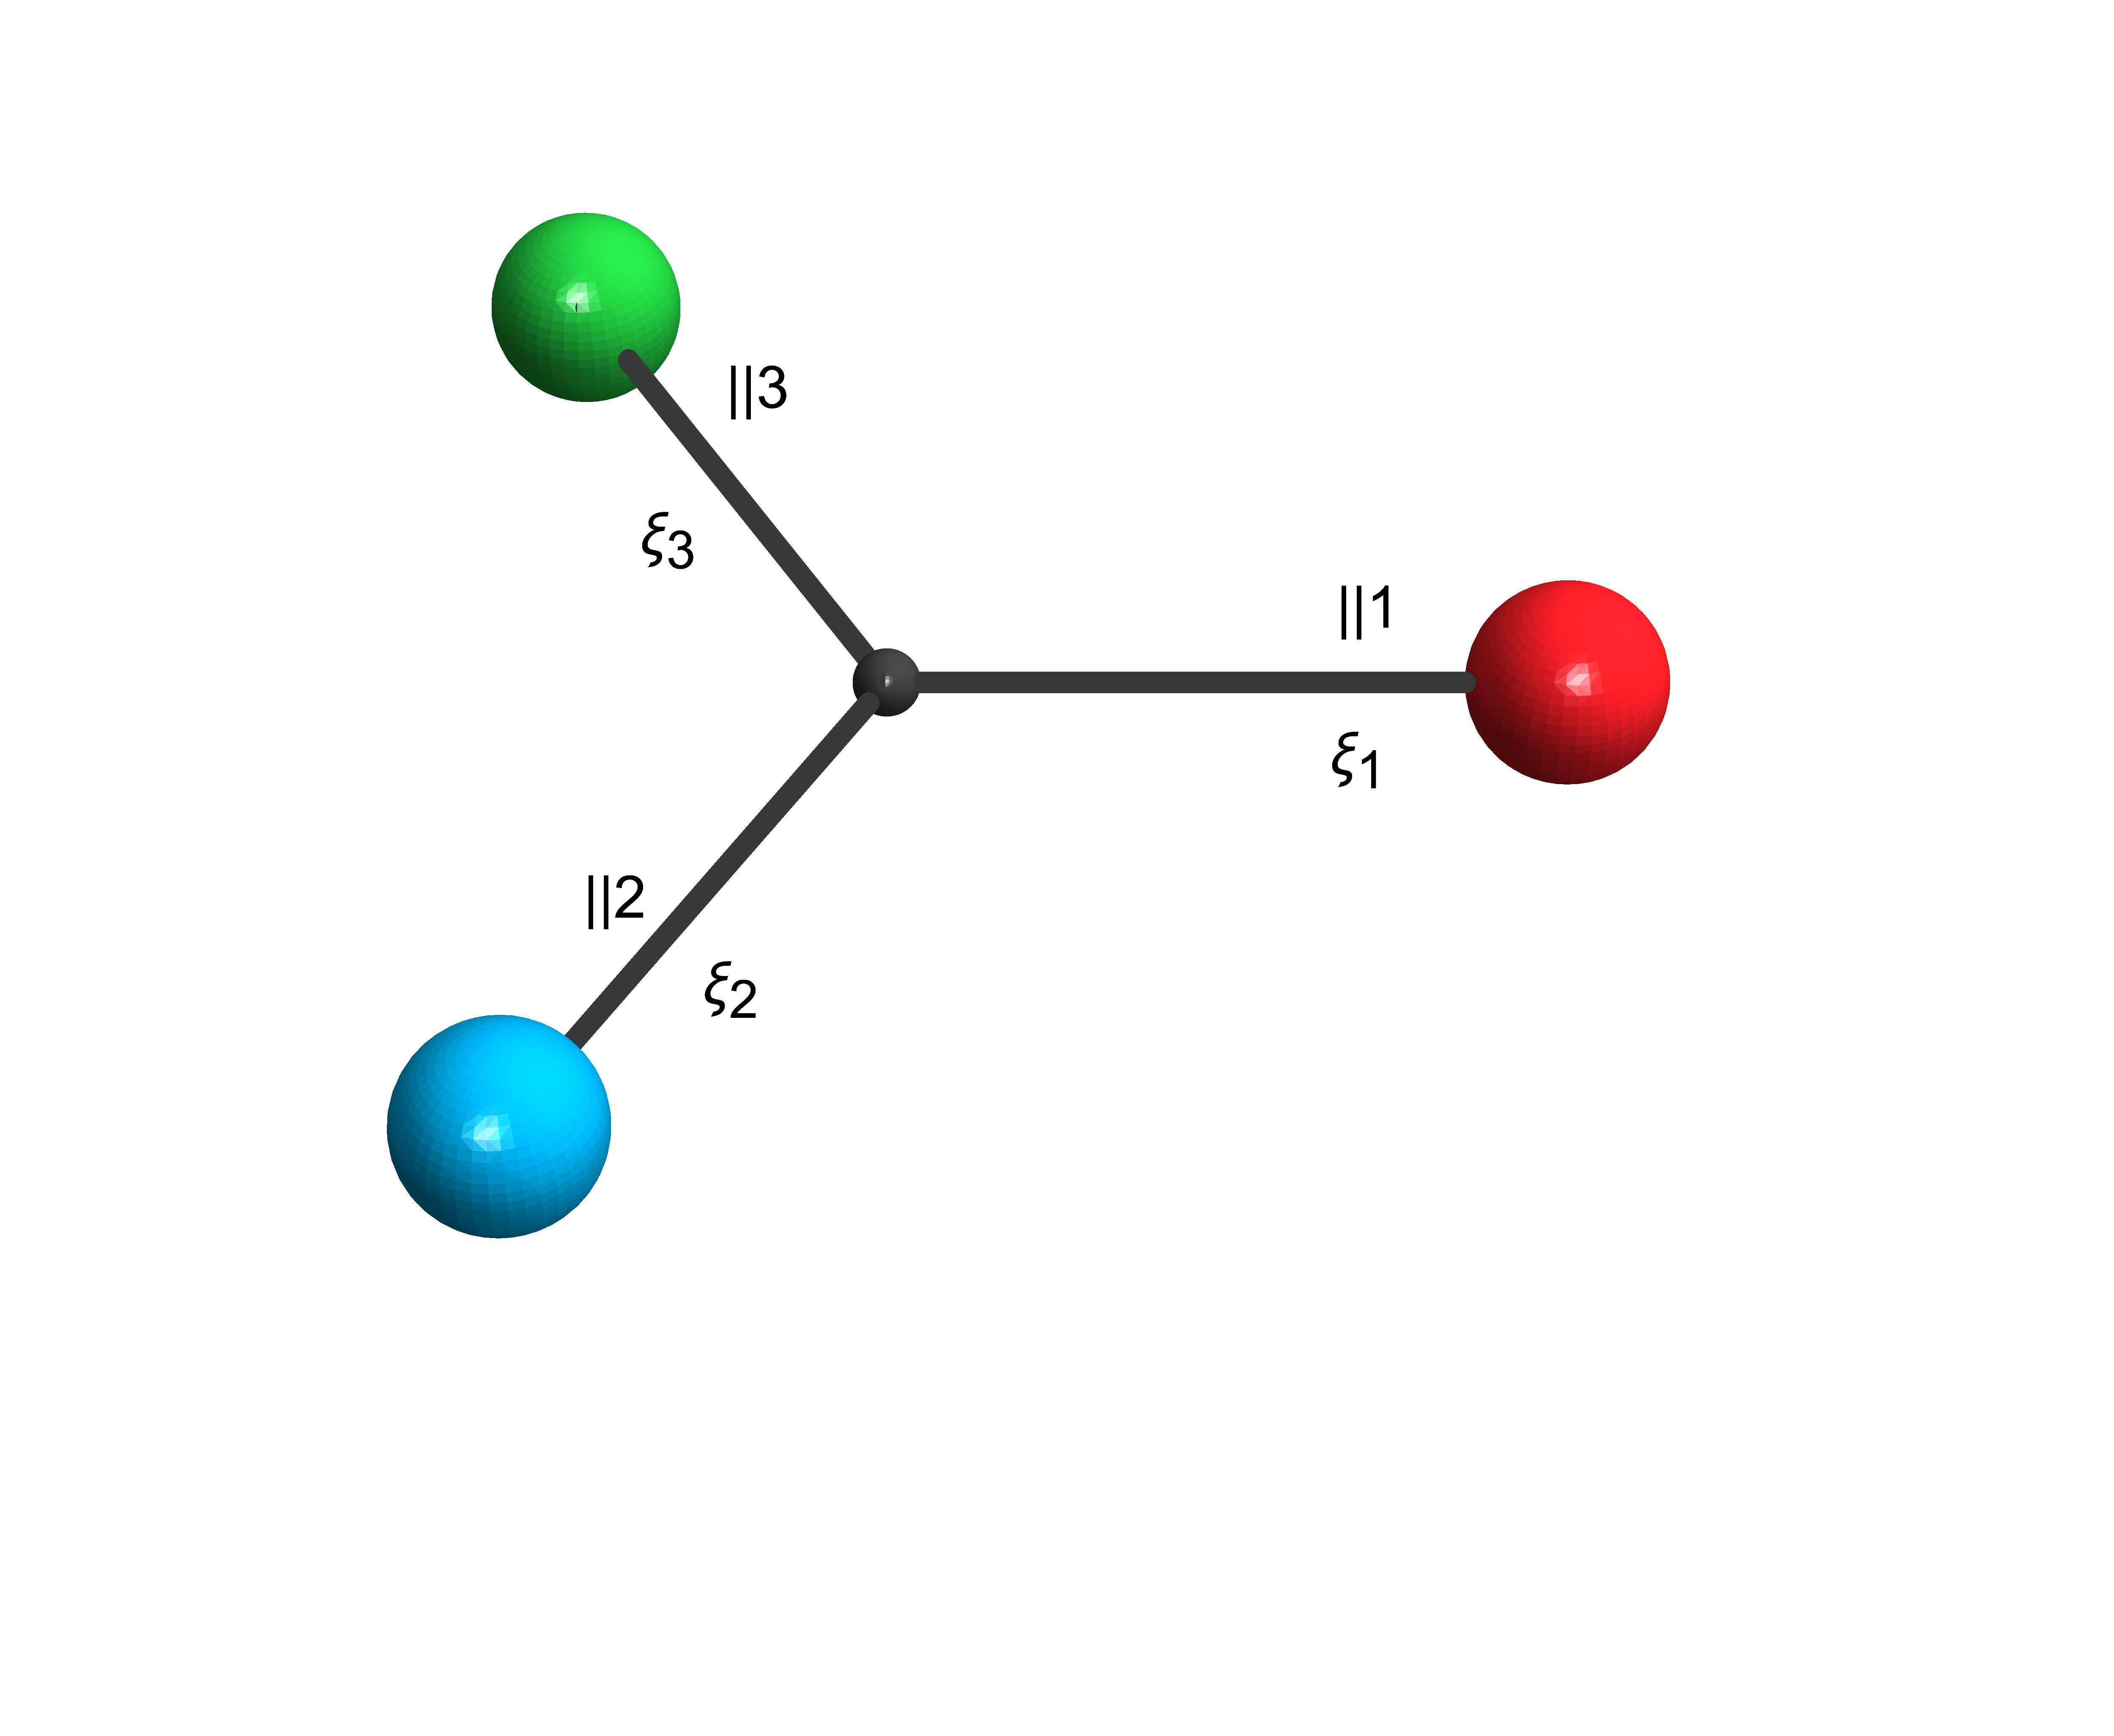
\includegraphics[scale=0.5]{/Users/philipp/Documents/GitHub/stage_cmap/images/spr3.png}
    \caption{The parking 3-sphere swimmer (\textsc{SPr3}) analyzed in \cite{Alouges2017}.}
    \label{fig:spr3}
\end{figure}

In \cite{Alouges2013}, a whole class of controllable micro-swimmer is presented. The said paper also puts forward a numerical method to address the problem of optimal swimming. However, their explicit dynamics as well as the structure of optimal swimming strokes remain largely unknown. In this paper, we will analyze further the swimmer \textsc{SPr4} from \cite{Alouges2013} and shed a light on the latter aspects. The analysis will take place very much in the spirit of the treatment of the swimmer \textsc{SPr3} in \cite{Alouges2017}, c.f. figure \ref{fig:spr3}, which originally had been presented in \cite{Alouges2013} as well. In fact, the swimmer \textsc{SPr4} is a natural generalization of the swimmer \textsc{SPr3}, capable of moving in the entire $3d$ space instead of just a plane. Although the principal techniques used in this paper are in close analogy to the ones in \cite{Alouges2017}, the more complex geometry of both the position and the shape space cause the analysis to be more involved.

Aim of this paper is to \emph{analytically} address the optimal control problem for \textsc{SPr4} in the range of \emph{small} strokes.

The rest of the paper is organized as follows: in section \ref{sec:modeling}, we give both a geometric and a kinematic description of parking 4-sphere swimmer (\textsc{SPr4}). Next, we introduce the control system treated in this paper. In section \ref{sec: symmetries}, we study the geometric structure of the control system taking advantage of the symmetries it has to satisfy due to the underlying Stokes  equations. In section \ref{sec: linearization}, we unravel the properties of the control system in the range of small strokes. Eventually, section \ref{sec: optimization} addresses the characterization of energy minimizing strokes for a special class of prescribed net displacements.




